\documentclass{article}
\usepackage{natbib}
\usepackage{graphicx}
\bibliographystyle{plainnat}
\usepackage{fancyheadings}
\usepackage{tabularx}
\usepackage{alltt, parskip, boxedminipage}
\usepackage{makeidx, multirow, longtable, tocbibind, amssymb}
%\usepackage{fullpage}
\makeindex
\usepackage[usenames]{color}
\definecolor{darkblue}{rgb}{0,0.05,0.35}

\usepackage[dvips, pagebackref, pdftitle={}, pdfcreator={epydoc 2.1}, bookmarks=true, bookmarksopen=false, pdfpagemode=UseOutlines, colorlinks=true, linkcolor=black, anchorcolor=black, citecolor=black, filecolor=black, menucolor=black, pagecolor=black, urlcolor=darkblue]{hyperref}
\setlength{\textheight}{21.5cm}
\setlength{\textwidth}{18cm}
\setlength{\hoffset}{-3.0cm}
\setlength{\footskip}{1.5cm}
\setlength{\headsep}{2.5cm}
\setlength{\voffset}{-2.5cm}
\newlength{\BCL} % base class length, for base trees.

\usepackage{everyshi}
 \makeatletter
 \let\totalpages\relax
 \newcounter{mypage}
 \EveryShipout{\stepcounter{mypage}}
 \AtEndDocument{\clearpage
    \immediate\write\@auxout{%
     \string\gdef\string\totalpages{\themypage}}}
 \makeatother

\newcommand{\esofooter}{
\includegraphics[height=1cm]{durlogo.eps}
{\bf \large Centre for \AA dvanced Instrumentation}
}
\newcommand{\esoheaderl}{
\includegraphics[height=1cm]{durlogo.eps}
\begin{tabularx}{9cm}{c}
\Large {\bf \esotitle} \\ \large {\bf(\esodoctype)}\\
\rightmark\hspace{0.1cm}
\end{tabularx}
\vfill
}
\newcommand{\esoheaderc}{
}
\newcommand{\esoheaderr}{
\begin{tabular}{|l|l|}\hline
Doc. number: & \esodocno \\ \hline
Release date: & \esoreleasedate \\ \hline
Issue number: & \esoissue \\ \hline
Page number: & Page \thepage \ of \totalpages \\ \hline
Author(s) & \esoauthorname \\ \hline
\end{tabular}


}

\pagestyle{fancy}
\cfoot[]{}
\lfoot[\esofooter]{\esofooter}
\lhead[\esoheaderl]{\esoheaderl}
\chead[\esoheaderc]{\esoheaderc}
\rhead[\esoheaderr]{\esoheaderr}
\renewcommand{\sectionmark}[1]{\markboth{#1}{#1}}

\newenvironment{Ventry}[1]%
  {\begin{list}{}{%
    \renewcommand{\makelabel}[1]{\texttt{##1:}\hfil}%
    \settowidth{\labelwidth}{\texttt{#1:}}%
    \setlength{\leftmargin}{\labelsep}%
    \addtolength{\leftmargin}{\labelwidth}}}%
  {\end{list}}

\newcommand{\mod}[1]{\texttt{#1}}
\begin{document}
\include{dummiestitle}
\thispagestyle{empty}
%This next command provides the CVS tag.  If you want a cvs tag on
%your document, add the following line at the start of the document,
%after replacing the & signs with dollar signs...
%\newcommand{\cvsID}{& &Id& (CVS)&}
\providecommand{\cvsID}{CVS ID not provided: document made on \today}

\begin{center}
\includegraphics{durlogo.eps}
\end{center}
\vspace{0.5cm}
\Huge
\begin{center}
\esoproject\\
\end{center}
\Large
\vspace{1cm}


{\bf 
\begin{tabular}{ll}
Document title: & \esotitle \vspace{0.5cm}\\ 

Documentation number: & \esodocno \vspace{0.5cm}\\ 

Document type: & \esodoctype \vspace{0.5cm}\\ 

Issue number:& \esoissue \vspace{0.5cm}\\ 

Release date: & \esoreleasedate \\ 

\end{tabular}
}

\normalsize
\vfill

\begin{tabular}{|l|l|l|p{5cm}|}
\hline
Document & \esoauthorname & Signature &\\
prepared by & \esoauthortype & and date &\\ \hline
Document & \esoapprovername & Signature &\\
approved by & \esoapprovertype & and date &\\ \hline
Document & \esoreleasername & Signature &\\
released by & \esoreleasertype & and date &\\ \hline
Document & \esoreviewername & Signature &\\
reviewed by & \esoreviewertype & and date &\\ \hline
\end{tabular}

\small
%\begin{alltt}
\cvsID
%\end{alltt}
\normalsize
%\lfoot[\esofooter]{\esofooter}
%\lhead[\esoheaderl]{\esoheaderl}
%\chead[\esoheaderc]{\esoheaderc}
%\rhead[\esoheaderr]{\esoheaderr}
%\renewcommand{\sectionmark}[1]{\markboth{#1}{#1}}

\pagebreak



\begin{center}
\Large
{\bf Change record\\ \vspace{1cm}}
\normalsize
\esochangerecord
\end{center}
\vspace{2cm}

\begin{center}
\Large
{\bf Notification list\\ \vspace{1cm}}
\normalsize
\esonotificationlist
\end{center}

\pagebreak

\begin{center}
\Large
{\bf Acronyms and abbreviations\\ \vspace{1cm}}
\normalsize
\esoabbreviations
\end{center}

\pagebreak

\begin{center}
\Large
{\bf Applicable documents\\ \vspace{1cm}}
\normalsize

\esoapplicabledocs
\end{center}
\vspace{2cm}

\begin{center}
\Large
{\bf Reference documents \\ \vspace{1cm}}
\normalsize

\esorefdocs
\end{center}

\pagebreak
\tableofcontents
\pagebreak


\section{Introduction}
This guide is intended to allow a dummy to create an executable AO
simulation.  It does not guarantee that the simulation created will
have meaningful scientific results (unlikely, given that a dummy
created it).  The simulation created will be a python program, which
can be executed and should not raise any errors.  It also provides
details of how to run an existing example simulation, and how to
analyse this.

\subsection{Required tools}
To create an AO simulation, you will need the following tools:
\begin{itemize}
\item Large piece of paper (at least A4 recommended, with spare in case
  of mistakes, squared paper with 0.5~cm pitch is probably optimal)
\item Colour pencils or pens (you should have at least the same number
  of colours as computing nodes, and each colour should have a number
  of shades equal to the number of processors per computing node.
  Additionally, you will need a black pen or pencil).
\item A computing platform capable of running the simulation code
  (Unix)
\item The simulation libraries and code
\item A text editor
\end{itemize}
Alternatively, you can use the simsetup GUI, which is included in the
CVS source code for the simulation.  This is the recommended way of
setting up a simulation.

\section{Running an existing simulation}
To run an existing simulation, you first need to obtain the AO
simulation code from CVS.  To do this, you need to execute the
following commands (and this assumes you have a CVS account):
\begin{verbatim}
export CVSROOT=":pserver:ali@localhost:/cfai_sw"
ssh -L 2401:localhost:2401 -l cvsd -N aipc42.phyaig.dur.ac.uk
cvs login
#optional part
cd
mkdir cvsstuff
cd cvsstuff
#end of optional part
cvs checkout aosim
\end{verbatim}

Once you have downloaded the simulation, change directory into the
\texttt{aosim} directory.  Then enter the command \texttt{make}.
After building of the simulation has completed, change directory to
the \texttt{example/test2} directory.  Then enter the command
\texttt{python testrun-sci.py}.  This will start the simulation
running.  It will print a message telling you which port it has opened
(probably 9000, or there abouts).  Take a note of this port number.

If you are trying to run a simulation that has been created by the
\texttt{simsetup} GUI, you can simply use the \texttt{aosim} command,
passing the name of the file to be run.  Please see the simsetup
documentation for further details.

Once you have the simulation running, start the simctrl.py program,
which can be found in the \texttt{aosim/gui/simctrl/} directory.  When
this has started, click on the connect button and choose your
simulation from the list.  If a warning appears instead of a list, run
the portdict.py program, and restart your simulation.  Then, click the
``get plots'' button, (or the load button, and select the \texttt{aosim/gui/simctrl/datactrl.xml}
file).  You are now in a position to analyse the simulation, and
various plots and controls can be obtained using the list of buttons
that appeared after loading the \texttt{datactrl.xml} file.  Further
details of this GUI are found in \citet{simctrlgui}.

\section{Simulation design}
\subsection{Creating a schematic design}
It is recommended that you use the \texttt{simsetup} GUI for
simulation creation.  Alternatively, you can follow the instructions
in the rest of this section.  However, please note, that you will be
offered no support if you choose to do things the hard way.  Please
use the \texttt{simsetup} GUI and then proceed to the
\ref{sect:paramfile} section (``Setting up the parameter file'') in
this document.

The first step to creating a simulation is to draw on a piece of paper
the schematic of the system that you wish to simulate.  When making
this drawing, you should place simulation modules (for example phase
screen generation, centroiding, science calculation) at least 2~cm
apart, surrounded by a box, and connect them with lines representing
the data flow between the modules.  If data is going into a module,
the line should attach to the top of the module box, while if it is
leaving a module, the line should attach from the bottom of the module
box.  An example sketch is shown in Fig.~\ref{fig:simsketch}.  Once
connected, place arrow heads on the lines, showing the direction of
the data flow.  This sketch should be drawn in a black pen.

\begin{figure}
\includegraphics[height=8cm]{pics/aosimsketchtrans.eps}
\caption{A sketch of an AO simulation}
\label{fig:simsketch}
\end{figure}

\subsection{Feedback}
Feedback (for example, passing reconstructor data back to a deformable
mirror) is implemented using either a specific \mod{feedback} module
for complex situations where large feedback latencies are required, or
using a science module developed with feedback in mind, for simple
cases with a single iteration feedback latency.  The reconstructor
modules have been designed with this option, and so can be used to
provide feedback.  This means that data can be obtained from them even
before they have processed anything at the start of the simulation
(i.e.\ the initialisation data is valid reconstructor values).  In
most (if not all) cases, you can simply connect the module requiring
feedback to the module providing the data.

\subsection{Multi-processor simulations}
You are now in a position where you can use your coloured pencils.
First, think about which modules you want to run on which nodes.  You
should consider the amount of data that needs to be passed between
nodes, and the amount of computing that needs to be done on a node,
and optimise the positioning of modules to minimise bottlenecks.  Once
you have done this, colour each module with a different colour
according to which node it will be placed on.  Then, if each node has
multiple processors (such as the Cray XD1, where each node is an SMP
machine with two processors), assign the modules onto different
processors using a different shade of the same colour, as shown in
Fig.~\ref{fig:simnodes}.  

\begin{figure}
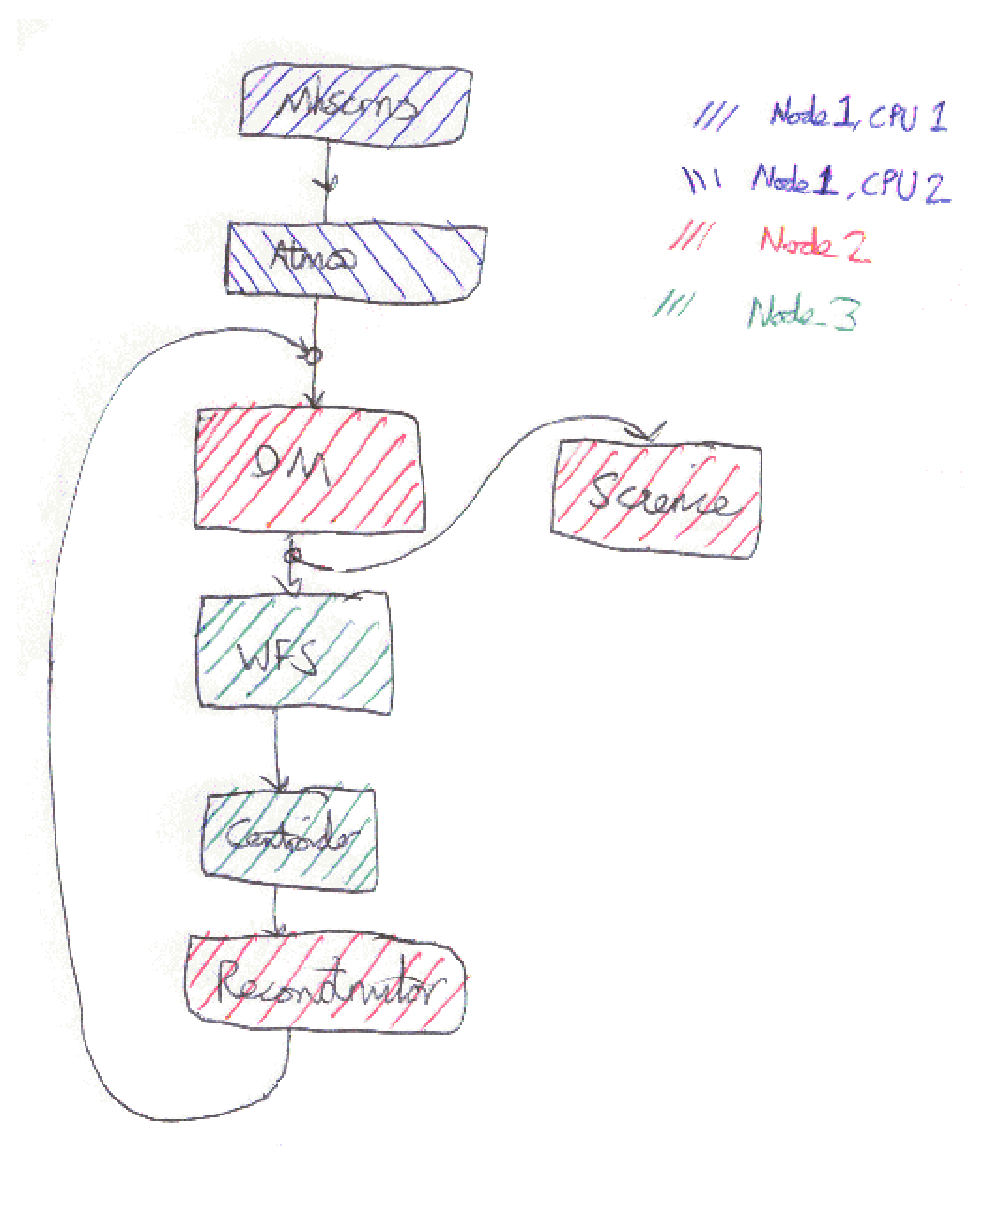
\includegraphics[height=8cm]{pics/aosimsketchnodestrans.eps}
\caption{A sketch of an AO simulation placed on different processing nodes}
\label{fig:simnodes}
\end{figure}


\subsubsection{Communication modules}
Now that you have placed the modules on different processors, you need
to consider how they will interact and communicate.  This is done
using the shared memory and MPI objects, \mod{shmGet}, \mod{shmSend},
\mod{mpiGet} and \mod{mpiSend}.  At each place where data flows
between two different coloured modules, place a \mod{mpiSend} and
\mod{mpiGet} module pair.  The \mod{mpiSend} module should be placed
on the processor which is generating the data, and the \mod{mpiGet}
module should be placed on the processor which is receiving the data.

SHM is faster than MPI for communications between processors within a
node (untested), and so is best used here.  SHM cannot be used for
communication with different nodes.

Next, at each point where data flows between modules with different
shades of the same colour, place a \mod{shmGet} and \mod{shmSend}
module pair.  The \mod{shmSend} module should be placed
on the processor which is generating the data, and the \mod{shmGet}
module should be placed on the processor which is receiving the data.

An example of a connected communicating simulation schematic is shown
in Fig.~\ref{fig:simcomms}

\begin{figure}
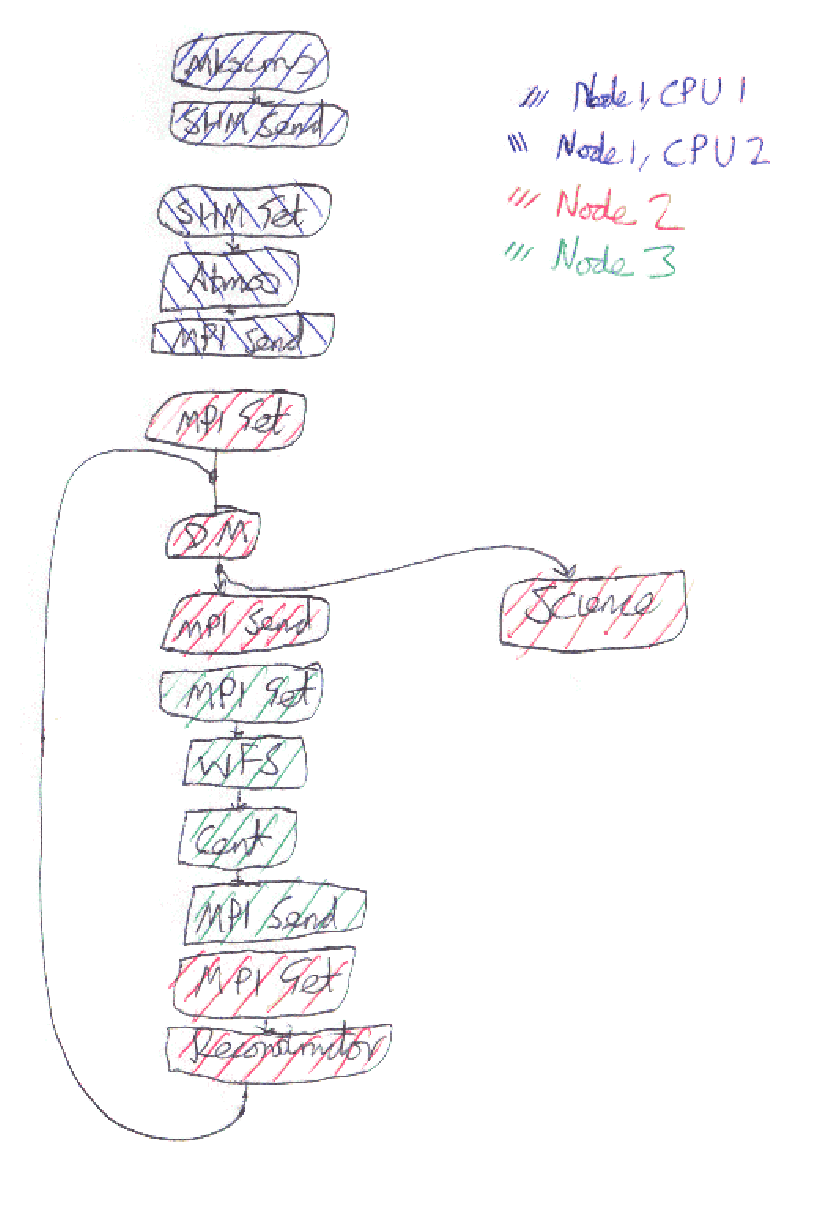
\includegraphics[height=12cm]{pics/aosimsketchcommstrans.eps}
\caption{A sketch of an AO simulation using MPI and shared memory
communication.}
\label{fig:simcomms}
\end{figure}

\subsection{Finalising the design}
You are now nearly ready to convert your design into electronic
format.  However, first, you must tidy up the design and finish off
some loose ends.

\subsubsection{The computation list}
Each process (on each node and processor) requires a list which
defines the order in which the computations for different modules are
carried out.  This may or may not be the same as the order from which
the modules obtain data from each other, depending on your situation.
In a simple case, this list will simply represent the order in which
the data flows.  One special case which may arise fairly commonly is
when feedback data is sent over a MPI or SHM connection.  In this
case, the connection object (\mod{mpiSend} or \mod{shmSend} module)
should be ordered to execute somewhere nearer the start than the
object whose feedback it is sending, to ensure that initial feedback
is sent.

The computation list for the node 2 example shown in Fig.~\ref{fig:simcomms}
could be
\begin{verbatim}
[MPI Get, Dm, MPI Send, Science, MPI Get, Reconstructor]
\end{verbatim}

\subsubsection{SHM efficiency considerations}
There is one final check that needs to be done before your diagram is
complete.  If you have several \mod{shmGet} modules receiving the same
data but from different \mod{shmSend} objects, then you should realise
that since the data can be shared, it can be implemented using a
single \mod{shmSend} object, supplying several \mod{shmGet} objects.

\subsection{Design completion}
Your simulation design is now complete.  Write your name and the date
in the bottom right hand corner.  You are now ready to convert the
design to electronic format.

\section{Simulation file creation}
\label{sect:simfilecreation}
To create a simulation file, make sure that you have your schematic
design ready.  Open a file in your favourite text editor (e.g.\ emacs
or vi), and give it a ``.py'' filename extension

\subsection{Importing necessary modules}
At the top of this file, import the various science modules you intend
to use, the \mod{Ctrl} module and possibly the \mod{feedback} module,
 for example: 

\begin{verbatim}
import util.Ctrl
import science.mkscrns 
import science.atmos
...
\end{verbatim}

You may also find it necessary to import the \mod{Numeric} module if
you wish to place an array into any feedback loops for the initial feedback.
To do this, type \texttt{import Numeric}.  Additionally, if you are
using multiple processors, you should import the MPI and shared memory
modules:

\begin{verbatim}
import base.mpiGet
import base.mpiSend
import base.shmGet
import base.shmSend
\end{verbatim}

Create a control object by typing
\texttt{ctrl=util.Ctrl.Ctrl(globals=globals())}.  This is used to
control the simulation.  The name of this object (ctrl) is important
because this is used by the simulation control GUI, and is assumed to
be as given.

\subsection{Separating the different processes}
If you are using a multiple process simulation, you can now write
skeleton text to separate the code to be executed on different
processors and nodes.  An example for a four processor simulation
could be written as follows:

\begin{verbatim}
if ctrl.rank==0:
    pass
elif ctrl.rank==1:
    pass
elif ctrl.rank==2:
    pass
elif ctrl.rank==3:
    pass
\end{verbatim}

You can determine the number of different processors used in your
schematic diagram by counting the number of different colours and
shades of colour used.  The example in Fig.~\ref{fig:simcomms} uses
4 different processors.  The \texttt{ctrl.rank} values are the MPI
rank of the process, and are obtained from a
\texttt{Scientific.MPI.World} object.

\subsection{Inserting simulation code}
You are now ready to replace the \texttt{pass} command with the
commands required to set up and run your simulation.  Some examples
will now follow.

\subsubsection{Phase screen generation example}
To have a module generating phase screens, and passing them to an MPI
connection on two other nodes, you could use:

\begin{verbatim}
#create the phasescreengeneration object
Mkscrns=science.mkscrns.mkscrns(None,ctrl.config)
#now create the shared memory array
shmInfo0=base.shmSend.shmInfo("/phsscrn",Mkscrns.outputData.shape,
                              Mkscrns.outputData.typecode(),nChild=1)
shmSend0=base.shmSend.shmSend(Mkscrns,shmInfo0)
#Specify the operation order, and start the main loop
ctrl.mainloop([Mkscrns,shmSend0])
\end{verbatim}

Use this code to replace the \texttt{pass} statement after the
\texttt{if ctrl.rank==0:} statement.

\subsubsection{Closed loop operation (Shack-Hartmann case)}
Now that we have generation of atmospheric phase screens, we need to
produce code to use them, first creating the pupil phase screen at a
given instance in time for a source in a given direction.  To do this
we would need:

\begin{verbatim}
#create a temporary object to get screen size from
m=science.mkscrns.mkscrns(None,ctrl.config,forGUISetup=1)
shmParent1=base.shmGet.shmParent("/phsscrn",m.outputData[0],m.outputData[1],0,1)
#delete the temporary object
del(m)
#create the shared memory communicator
shmGet1=base.shmGet.shmGet(shmParent1)
Atmos=science.atmos.atmos(shmGet1,ctrl.config,debug="Atmos")
mpiInfo=base.mpiSend.mpiChild(2,90)
#create the MPI communicator
mpiSend1=base.mpiSend.mpiSend(Atmos,mpiInfo,ctrl.mpiComm,debug="mpiSend1")
#specify the operation order, and start looping
ctrl.mainloop([shmGet1,Atmos,mpiSend1])
\end{verbatim}

Use this code to replace the \texttt{pass} statement after the
\texttt{elif ctrl.rank==1:} statement.

\subsubsection{Science targets}
We now have atmospheric pupil phase screens, and so want a fully
working AO system with closed loop operation.  We also wish to derive
science parameters (such as Strehl ratio) from the target.  Some of
this will be accomplished now.  However, we will do wavefront sensing
and centroiding on yet another node, for demonstration purposes.

\begin{verbatim}
#A temporary atmos object, to get the size of phase screens.  
a=science.atmos.atmos(None,ctrl.config,forGUISetup=1) #Note the use of the forGUISetup flag.
mpiscrninfo1=base.mpiGet.mpiParent(a.outputData[0],a.outputData[1],1,90)
del(a)
#Get the phase screens.
mpiGet1=base.mpiGet.mpiGet(mpiscrninfo1,ctrl.mpiComm,debug="mpiGet1")
#Set up the deformable mirror
Dm=science.el_dm.dm({"atmos":mpiGet1},ctrl.config,debug="Dm")
#Send deformed phase screens to another process
mpiSend2=base.mpiSend.mpiSend(Dm,base.mpiSend.mpiChild(3,91),ctrl.mpiComm,debug="mpiSend2")
#in parallel with computing the science.
sci=science.science.science(Dm,ctrl.config,debug="sci")
#a temporary object to get the centroid data size
c=science.cent.cent(None,ctrl.config,forGUISetup=1)
mpiscrninfo2=base.mpiGet.mpiParent(c.outputData[0],c.outputData[1],3,92)
del(c)
#receive the centroided values from another process.
mpiGet3=base.mpiGet.mpiGet(mpiscrninfo2,ctrl.mpiComm,debug="mpiGet3")
#Apply reconstruction algorithms to reshape the deformable mirror.
Recon=science.el_recon.recon(mpiGet3,ctrl.config,debug="Recon")
#Now that the reconstructor object has been created, we can update the
#DM dictionary, so that it knows where to receive reconstructor data from.
Dm.parent["recon"]=Recon
#Specify the execution order, and start looping.  Note the implicit
#use of feedback here:  The Dm object will read data from the Recon
#object before the Recon object has been executed for the first time,
#and hence will continually read data from the previous iteration.
ctrl.mainloop([mpiGet1,Dm,mpiSend2,sci,mpiGet3,Recon])
\end{verbatim}

Use this code to replace the \texttt{pass} statement after the
\texttt{elif ctrl.rank==2:} statement.  For the wavefront sensing and
centroiding, we could have:

\begin{verbatim}
#temporary object to get phase screen size
d=science.el_dm.dm(None,ctrl.config,forGUISetup=1)
mpiscrninfo3=base.mpiGet.mpiParent(d.outputData[0],d.outputData[1],2,91)
del(d)
#receive data from the DM
mpiGet2=base.mpiGet.mpiGet(mpiscrninfo3,ctrl.mpiComm,debug="mpiGet2")
#convert to CCD images
Wfs=science.wfs.wfs(mpiGet2,ctrl.config,args={"fpprecision":32},debug="Wfs")
#compute centroids
Cent=science.cent.cent(Wfs,ctrl.config,debug="Cent")
#send centroids back to the receiving process (rank 2)
mpiSend3=base.mpiSend.mpiSend(Cent,base.mpiSend.mpiChild(2,92),ctrl.mpiComm,debug="mpiSend3")
#specify execution order and start looping
ctrl.mainloop([mpiGet2,Wfs,Cent,mpiSend3])
\end{verbatim}

Use this code to replace the \texttt{pass} statement after the
\texttt{elif ctrl.rank==3:} statement.

\subsection{Likely errors}
If you find that when you come to run a simulation file that you have
created, it does not work, there are several likely sources of error.
The first is that not all your Send modules (e.g.\ \mod{mpiSend} and
\mod{shmSend}) are in the execution list.  You should also check that
you have imported all the necessary modules.  It is acknowledged that
setting up the simulation file is not trivial.  Please bear in mind
that most of the time, you are also not trying to simulate something
trivial, and so you should be sure to understand what you are trying
to do, and the way in which the simulation framework works, as this
will save you a lot of time later on.  The example given here covers
all parts of the framework, so should give some help.

There is generally a mixed feeling about whether a graphical user
interface should be created to allow simulations to be created using
point-and-click techniques.  Some feel that creating such a GUI would
be a waste of time, while others feel that it would greatly aid
setting up the simulations, which for larger simulations can be
complicated.  At the moment, there is no plan to create such a GUI,
however if you have any comments about this, please let the simulation
team know.

\section{Setting up the parameter file}
\label{sect:paramfile}
You now have a simulation file that can be run by the python
interpreter.  However, before doing this, you must create the
parameter file, either using paramgui.py or editing an XML parameter
file by hand in a text editor.  It is recommended that you use the
paramgui.py program for this purpose. 

For the example here, you would need to create modules for mkscrns,
atmos, el\_dm, wfs, cent, el\_recon and
science.  This process, though straightforward, may take a while.
Further details are given in \citet{simparamgui}, and about the
parameter file format in general in \citet{overview}.



\section{Running the simulation}
Once the parameter file is set up, you are ready to run the
simulation.  This can be done by executing the following command:

\begin{verbatim}
aosim mysimulation.py --param-file=\$PWD/myparams.xml
or
aosim mysimulation.py
(if your parameter file is called params.xml in the same directory).
\end{verbatim}

Or, if you have set up the simulation the hard way, without using the
\texttt{simsetup} GUI, you should type:
\begin{verbatim}
mpirun -np 4 -hostlist node1 node1 node2 node3 /usr/local/bin/mpipython \
$PWD/mysimulation.py --param-file=\$PWD/myparams.xml
\end{verbatim}

This assumes that you are in the same directory as the simulation
python file (named mysimulation.py) and the parameter XML file (named
myparams.xml), and that the mpipython executable can be found in
/usr/local/bin/.  Note, that if you don't use the
\texttt{--param-file} switch, a parameter file called
\texttt{params.xml} will be used by default, if it exists in the
current directory.  It also assumes that the three nodes you wish to
run the simulation on are called node1, node2 and node3.  Note that
the first two processes must be on the same node as the communicate
using shared memory.

\subsection{Command line arguments}
There are a number of command line arguments that can be passed to a
simulation.  These include
\begin{enumerate}
\item -h or --help to display a help message (including an up to date
  list of command line arguments).
\item --start-paused to place the simulation in an initial paused
  state.
\item --param-file=FILENAME to specify a parameter file name (the
  default is params.xml).
\item --iterations=N to specify the number of iterations the simulation
  is run for (the default is infinity if not specified in the
  parameter file).
\item --param=''python text string'' to change a parameter on the fly,
  for example, you could use --param=''this.globals.wfs\_n=16'' to
  change the value of wfs\_n to 16, but without having to change the
  parameter file.  Note, this should be used with care, because there
  will probably be no record of the change (unless the commandline
  switch is saved).
\item --batchno=VALUE can be used to run a specific batch (specific
  parameters from the parameter file, as chosen by you).
\end{enumerate}

If you are doing things without the \texttt{simsetup} GUI, when you
have determined the correct way in which to run your simulation, it is
suggested that you add the command as a string at the top of the file,
so that you will be able to re-run it at a later date.  This command
can also be written into a shell script.  To do this, you should do
the following at the command line:
\begin{verbatim}
cat > myscript.sh
NOW PASTE THE COMMAND INTO THE BUFFER
TYPE CTRL-D
chmod +x myscript.sh
\end{verbatim}

\section{Controlling the simulation}
Once you have a running simulation, you may connect to it, to analyse
and debug it, and to display plots of any data you are interested in.
To do this, use the simctrl.py GUI.  After the GUI has started, you
should first connect to every process that is part of the simulation,
giving the hostname and port number that you wish to connect to.  By
default, the simulation processes will be listening on port number
9000 plus their MPI rank (so for a four process simulation you should
connect to ports 9000, 9001, 9002 and 9003 on the respective nodes on
which the processes are running).  If for any reason, the simulation
process was unable to open a listening port at this port number (for
example, someone else was running a simulation which had taken this
port), it will increase the port number by the total number of
processes running in your simulation (four in this case) and try
again.  This will repeat until it is able to open a port successfully.

Further details about the simulation control GUI are given in
\citet{simctrlgui}

\section{Setting up your own module}
If you wish to create your own science module, the following skeleton
should be used.  Additionally, rules, as defined in \citet{overview},
should be adherred to.

\begin{verbatim}
#A sample science module skeleton.
"""$Id (place a $ symbol after id so that CVS labels it correctly)
My science module
"""
import base.aobase
import Numeric
#now import everything else you'll need.
class myscience(base.aobase.aobase):
    """My science object.  Correct documentation, compatible with
    epydoc goes here, including information about class variables. e.g.
    @cvar parent: The parent object
    @type parent: Object
    """
    def __init__(self,parent,config,args={},forGUISetup=0,debug=None):
        """Initialise my object.  Give details (compatible with
        epydoc about the input arguments here.  e.g.
        @param parent: A parent object
        @type parent: Object
        """
        base.aobase.aobase.__init__(self,parent,config,args,forGUISetup,debug)
        self.parent=parent
        #Now read any values from the configuration file. e.g.
        self.myvalue=config.getVal("myvalue")

    def generateNext(self,msg=None):
        """Place your computation here.  Use self.parent.outputData to obtain
        the data from the predecessor (parent) module, and place your
        result in self.outputData.
        If you need to change self.parent.outputData, make a copy
        first.
        You should be careful about validData flags, see other
        examples for details.
        """
        self.outputData=myfunction(self.parent.outputData)
        return self.outputData

    def plottable(self):
        """XML string for GUI use"""
        return """<plot title="my data" cmd="data=$OBJ.outputData" ret="data" type="gist"
                   when="rpt"/>"""

    def getParams(self):
        """parameters required for this module"""
        return {"myvalue":99.8,"myothervalue":99.7}

    def getInputType(self):
        """Returns the input needed by this module.
        Should return an instance of dataType, or a list of dataType objects,
        or None if no input is required."""
        return base.dataType.dataType("My required input",Numeric.ArrayType,(10,10),Numeric.Int32)

    def getOutputType(self):
        """Returns the output given by this module."""
        return base.dataType.dataType("my output",Numeric.ArrayType,(20,20),Numeric.Float32)

    def getInitArgs(self):
        """return a dictionary of parameters that can be passed to init.
        Dictionary key is the parameter name, and dictionary value is a tuple
        of (description, default value).  If there is no default value, then
        the dictionary value is a tuple of (description,).
        """
        return {"parent":("Predecessor object",),"config":("Configuration object",),
                "args":("Optional arguments",{}),"forGUISetup":("initialisation type",0)}

\end{verbatim}

\subsection{Short cuts}
There are several shortcuts or handy hints which can be implemented
when running a simulation.  The first is to use the batch facility in
cases where a parameter space has to be explored.  By setting up a
variable in the parameter file which depends on batch number, a number
of different simulations can then be run just by using a different
batch number (use --batchno=XXX on the command line).

When you wish to run a large number of simulations which require user
input, e.g.\ to poke the deformable mirror and hence compute a poke
matrix, this can become tedious.  The use of the
\texttt{initialCommand} method in the control object can then be used
to automate these inputs, by giving commands to the simulation which
can be executed after a given iteration.  So, for example, you might
use this to open the loop and start a poke at iteration zero.  Then at
a number of iterations later, you might close the loop and start the
real simulation.  This then means that the simulation can be run
without user intervention from start to finish.  

Finally, if you wish to create some statistics from a number (e.g. 10)
of runs of the same simulation (so that you can for example find an
error estimate for the computed Strehl ratio etc), you can create a
simple bash script which will run all the simulations for you.  This
of course will only work if the simulation requires no user
intervention between start and finish.  For an example of this, look
in the \texttt{projects/ali/glao/runglao.sh} script.  This script
takes 2 commandline arguments, the batch number, and the number of
simulations to run.  This is then good for building up statistics.


\appendix
\section*{Appendix 1:  A complete simple simulation code}
It doesn't need to be all that difficult.  This example performs
closed loop operation with the adaptive optics correction reference
target being the same as the science target, and runs as one process.
This example is from aosim/example/test2/newtest-sci.py
\begin{verbatim}
import science.mkscrns
import science.atmos
import science.el_dm
import science.wfs
import science.cent
import science.el_recon
import science.science
import util.Ctrl
import Numeric
ctrl=util.Ctrl.Ctrl(globals=globals(),debug="ctrl")
#set up the science modules
Mkscrns=science.mkscrns.mkscrns(None,ctrl.config)
Atmos=science.atmos.atmos(Mkscrns,ctrl.config)
Dm=science.el_dm.dm({"atmos":Atmos},ctrl.config)
Wfs=science.wfs.wfs(Dm,ctrl.config,args={"fpprecision":32})
Cent=science.cent.cent(Wfs,ctrl.config)
Recon=science.el_recon.recon(Cent,ctrl.config)
Dm.parent["recon"]=Recon
Sci=science.science.science(Dm,ctrl.config)
execOrder=[Mkscrns,Atmos,Dm,Wfs,Cent,Recon,Sci]
ctrl.mainloop(execOrder)#start the main simulation loop
\end{verbatim}

\section*{Appendix 2:  The complete simulation code for the example
  given in this document}
\begin{verbatim}
See the aosim/example/test2/dummy.py example
\end{verbatim}

\pagebreak
\bibliography{references}

\printindex
\end{document}
